\documentclass{article}
\usepackage{natbib} % Bibliography
\bibpunct{(}{)}{;}{a}{}{;} % Bibliography
\setcitestyle{authoryear,open={},close={}} % Use 'It was found that something is something (Name 1234)' style

% Comments
\newcommand*\rampal[1]{\textcolor{red}{\textbf{[RSE: #1]}}}
\newcommand*\richel[1]{\textcolor{orange}{\textbf{[RJCB: #1]}}}
\newcommand*\gio[1]{\textcolor{blue}{\textbf{[GL: #1]}}}

% Packages
\usepackage{amssymb}
\usepackage[english]{babel}
\usepackage{bbm}
\usepackage{dsfont}
\usepackage{setspace} % Use double spacing
\doublespacing % Use double spacing
\usepackage{pgf}
\usepackage{hyperref}
\usepackage{verbatim}
\usepackage{comment}
\usepackage{lineno} % Adds numbered lines
\linenumbers % Adds numbered lines

\hyphenation{
  BEAST
  Pa-ra-me-ter
  Drum-mond 
  Bayes-ian 
  Mr-Bayes 
  ap-proach-es 
  Rev-Bayes 
  cre-ate
  spe-ci-a-tion-com-ple-tion
  pro-trac-ted
 }

\usepackage{authblk}
\title{The error in Bayesian phylogenetic reconstruction when speciation co-occurs}

\author[1]{Giovanni Laudanno}
\author[1]{Rich\`el J.C. Bilderbeek}
\author[1]{Rampal S. Etienne}
\affil[1]{Groningen Institute for Evolutionary Life Sciences, University of Groningen, Groningen, The Netherlands}


\begin{document}

\maketitle

\begin{abstract}
% From 'How to construct a Nature summary paragraph'

% A short abstract of fewer than 200 words is acceptable.

% One or two sentences providing a basic
% introduction to the field,
% comprehensible to a scientist in any discipline.
There exist millions of species on Earth,
all originating from a common ancestor billions
of years ago.
The field of phylogenetics uses heritable material (e.g. DNA)
to determine the evolutionary history of species.

% Two to three sentences of
% more detailed background, comprehensible to
% scientists in related disciplines.
Starting from heritable material and explicit assumptions,
Bayesian phylogenetics allows to infer a jointly-estimated 
phylogeny and parameter estimates distribution.
One of these assumptions in the speciation model, which
mathematically describes the branching process of a phylogeny in time.
The most used speciation model assumes that speciation events are
independent, where we know that certain events can trigger speciation 
events in multiple species.

% One sentence clearly stating the general
% problem being addressed by this particular
% study.
This research answers the question what the impact is of using a
species tree model that assumes speciation is independent, when it
is used on phylogenies created by a tree model in which speciation can
co-occur.

% One sentence summarising the main
% result (with the words “here we show”
% their equivalent).
Here we show the inference error made,
when nature has varying degrees of co-occurring speciation
over a wide range of parameter settings.

% Two or three sentences explaining what
% the main result reveals in direct
% comparison to what was thought to be the case
% previously, or how the main result adds to
% previous knowledge.
We show that the inference error correlates
with the amount of co-occuring speciation events,
which valudates

% One or two sentences to put the results into a
% more general context.
These results allow phylogeneticist to judge under which
circumstances the commonly used speciation model can be safely 
used. 

% Two or three sentences to provide a
% broader perspective, readily comprehensible
% to a scientist in any discipline, may be included
% in the first paragraph if the editor considers that the accessibility of the paper is significantly enhanced
% by their inclusion. Under these circumstances, the length of the paragraph can be up to 300 words.
In a bigger picture, these results showcase the use of a general and 
flexible method we used to assess the impact of using an oversimplistic tree 
prior, helping phylogeneticists to find the line between 'too simple'
and 'too complex' speciation models.

\end{abstract}

{\bf Keywords:} computational biology, evolution, phylogenetics, Bayesian analysis, tree prior,
pirouette, BEAST2, babette

\section{Introduction}

Modern computational techniques, such as BEAST (\citep{beast,beast2}), RevBayes (\citep{hohna2016revbayes}) and MrBayes (\citep{huelsenbeck2001mrbayes,ronquist2003mrbayes}), allow to infer phylogenetic trees from genetic data 
such as DNA, RNA or proteins.
They return posterior distributions of phylogenies 
and estimated parameters by running a Bayesian analysis, 
given aligned sequence data and a set of models. 
One of these models is the diversification model, for which a prior distribution must be provided. Within the Bayesian framework this is called a tree prior; it is a mathematical description 
of the probability distribution of possible branching patterns before looking at the data. Together with the signal from the data, this tree prior will determine the posterior distribution of phylogenies, i.e. after considering the data. Other models include the nucleotide substitution model (i.e. a model of relative transition rates between different nucleotides through time) and the clock model (a model determining the absolute rate of changes for each lineage). For each of these models choices must be made and prior distributions must be specified for their parameters. BEAST2 gives the user the option to set up 
several possible phylogenetic 
priors (e.g. substitution/clock/diversification models). 
However, currently available priors 
might be not suitable to analyze some specific datasets.
For this reason BEAST2 provides users with the possibility 
to introduce new models and corresponding priors. Particularly, one can specify the tree prior for a new model of diversification.

Current phylogenetic tools such as BEAST2 assume that 
only a single speciation event can occur at any given time.
This assumption is consistent with many different diversification models (e.g \cite{Maddison2007biSSE}, \cite{Valente2015}, 
\cite{etienne2012diversity}, \cite{etienne2014estimating}). However, multiple speciation events can take place simultaneously and repeatedly when populations are intermittently disconnected and connected, for example due to climatic fluctuations. This has been called the species pump hypothesis (\citep{haffer1969speciation}) and has been invoked particularly in mountainous areas that underwent glaciation (\citep{muellner2019origins}). Our own interest in the species pump hypotheses arose from its potential explanation of the radiation of cichlid fish in the African rift lakes (Malawi, Tanganyika and Victoria), where water level drops created multiple smaller lakes providing the opportunity for allopatric speciation in multiple species.  (\citep{verheyen1996mitochondrial}, \citep{sturmbauer2001lake}, \citep{janzen2017}).

One could study whether the species pump hypothesis is a viable explanation in empirical ystems by comparing divergence times of sister taxa (\citep{oaks2019comparative}). A more inclusive approach would involve using a model allowing multiple simultaneous speciation events as a new species tree prior in phylogenetic reconstruction. However, introducing a new tree prior may be computationally prohibitive (\citep{bilderbeek2019pirouette}), and may also not be necessary, as current standard birth death (BD) tree priors might prove to be good enough at inferring the correct tree. Here we use the R package \verb;pirouette; (\citep{pirouette}) to check whether this is the case by simulating phylogenies under a species pump model, i.e. the multiple-birth-death model (MBD), with the \verb;mbd; package (\citep{mbd}), then simulating sequence alignments for each of these trees and finally inferring a phylogenetic tree using BEAST2 from these alignment. By comparing the inferred phylogeny with the true (simulated) one, we measure the inference error made by adopting a standard BD tree prior.

\section{Methods}

\subsection{Simulation model}

The multiple-birth-death (MBD) model inherits the parameters $\lambda$ and $\mu$ from the BD model; they correspond, respectively, 
to the traditional per-species speciation and extinction rates. 
Additionally, the MBD model assumes that external events, occuring at rate $\nu$ triggers a speciation initiation event in each lineage which leads to a full new species with probability $q$. 
Whereas parameter $\lambda$ can be interpreted as the rate of sympatric speciation, $\nu$ is the rate of appearance of 
geographical barriers able to interrupt the gene flow in the population,
resulting in a possible allopatric speciation for each of the species.  
Even though multiple speciation events can occur simultaneouly, it does not lead to  
polytomies, because each species can only split once after a trigger event. This model can be easily simulated with a Doob-Gillespie algorithm. A probability distribution for the phylogeny under the MBD model can also be formulated using the integration approach developed for diversity-dependent diversification models \citep{etienne2012diversity}, which has been explored in \cite{mbd}.\rampal{Is this the mbd chapter?}. While this probability distribution could in principle be used as a tree prior in Bayesian phylogenetic inference, it is computationally very demanding, particularly for large trees. With the MBD model we generate simulated datasets for various parameter settings, using the \verb;mbd_sim; function from the \verb;mbd; R package [\citep{mbd}].

\subsection{Estimating the inference error}

From each simulated 'true' MBD tree, we measure the impact of
ignoring the more complex and non-standard MBD tree prior in
Bayesian phylogenetic inference with the R package \verb;pirouette; [\citep{pirouette}].
 \verb;pirouette; starts from a 'true'  phylogeny (in our case: the simulated MBD tree), and simulates a DNA sequence alignment on it using a known nucleotide substitution model and a clock model. 
From each sequence alignment, a Bayesian inference is run with a particular choice of tree prior and substitution and clock models. One can choose the same substitution and clock models as used in generating the tree, or pick the ones that fit the data best. For the tree prior we assume the BD model (as the effect of this choice is our focus). We obtain a posterior distribution of jointly-estimated trees and model parameter estimates.
By comparing the true tree and the posterior trees, an inference error distribution is generated. For this comparison we used the absolute nLTT statistic by \citet{janzen2015}, which results in an error distribution with values ranging from zero (when the inferred tree is identical to the true tree) to a maximum of one (trees are completely different).

We used the twinning option available in \verb;pirouette; that allows to quantify the impact of assuming a wrong tree prior in a Bayesian inference compared to a reference background error that would arise even if the models used in inference were identical to those used in generating the tree (i.e. the twin tree was generated with a BD model).

\giovanni{Add mention to Jensen-Shannon divergence metric, if used.}

\subsection{Parameter settings}

\iffalse
We ran multiple pilot experiments with 1 replicate to arrive at our final
parameter settings. We devised a set of rules to make a verdict about the
settings \richel{(script at \url{https://github.com/richelbilderbeek/razzo_project/blob/master/scripts/90_collect_run_times.R},
resulting verdicts at \url{https://github.com/richelbilderbeek/razzo_project/blob/master/verdict.md})}:
\begin{itemize}
  \item quality: 95\% of all individual runs should have an ESS of at least 200.
    \richel{figure \ref{fig:esses}}
  \item feasibility: 95\% of all individual runs should finish within 10 days.
    \richel{figure \ref{fig:runtimes}}
  \item reproducibility: the mean run-time of all finished runs should be less than 24 hours 
    \richel{I suggest}.
    \richel{figure \ref{fig:runtimes}}
  \item relevance 1: the percentage of taxa created by the MB process should be
    as high as possible
  \item relevance 2: the percentage of taxa should be
    as high as possible
\end{itemize}
We searched through parameter space until these criteria were met.
All the parameter settings used in the pilot experiments can be found at 
\url{https://github.com/richelbilderbeek/razzo_project/blob/master/overview.md}.
Due to the low number of replicates, we were unable (nor tried)
to draw conclusions based on the results.
\fi

When working with simulated datasets the choice of the generating parameters is always somewhat arbitrary. In principle one would choose a parameter range as wide as possible to characterize most of parameter space. However, both simulation and inference need to be possible computationally. To ensure this
we required the following criteria to be satisfied for a parameter set to be chosen: \giovanni{Does this apply only to the mbd parameters or also to the pirouette ones?}:
\begin{itemize}
  \item Quality: At least 95\% of all inferences should have an Estimated Sample Size (ESS) of at least 200 (see \cite{beast} for reference);
    \richel{figure \ref{fig:esses}}
  \item Feasibility: At least 95\% of all individual runs should finish within 10 days;
    \richel{figure \ref{fig:runtimes}}
  \item Reproducibility: the mean run-time of all finished runs should be less than 24 hours \richel{figure \ref{fig:runtimes}}
    
    \richel{I suggest}. \giovanni{What's the difference with the previous point?}
  \item Relevance 1: In order to have a meaningful inference, we demand that the MB signal is detectable to a satisfactory extent. For this reason the percentage of taxa created by the MB process should be as high as possible;
  \item Relevance 2: Small trees might not contain a significant amount of information to be analyzed. For this reason we demand that the number of taxa should be as high as possible, as long as all the other requirements are met;
\end{itemize}

This resulted in the simulation parameters in Table~\ref{tab:simulation_parameters}.

\begin{table}[ht]
  \centering
  \begin{tabular}{ | c | l | }
    \hline
    \textbf{Parameter} &
    \textbf{Values} \\ 
    \hline
    $\lambda$ & (0.2) \\
    $\mu$ & (0, 0.15) \\
    $\nu$ & (0.0, 0.5, 1.0, 1.5, 2.0) \\
    $q$ & (0.1, 0.15, 0.2) \\
    crown age & 6 \\
    \hline
  \end{tabular}
  \caption{
    Parameters used to simulate MBD trees. For each parameter setting $1000$ trees are simulated.
  }
  \label{tab:simulation_parameters}
\end{table}

We assumed that the alignments are 1000 nucleotides in length, with a known root sequence of four 250 mono-nucleotide blocks, generated using the simplest nucleotide substitution model (Jukes Cantor, JC69) and clock model (strict), with a mutation rate of $\frac{t_c}{2}$, where $t_c$ is the crown age. 
With this mutation rate, each nucleotide has a 50\% chance to mutate (both silently and non-silently) from the ancestral root sequence to any of the contemporary species' sequences at the tips.

For the Bayesian inference, we assumed a generative model of a JC69 site model, a strict clock model and a BD tree prior.
Additionally, we used a Most Recent Common Ancestor (MRCA) prior equal to the crown age with a normal distribution of width $\sigma = 0.01$. We used a Markov Chain Monte Carlo (MCMC) setup of $10^6$ states with a sampling interval of once per $10^3$ states. Of the resulting $10^3$ states, we discarded a burn-in of $10\%$.

To verify that the generative model (with a BD tree prior) is indeed the most appropriate standard model, we compared it to 39 other candidate inference models.
These candidate models are all other combinations of four tree priors, two clock models and five speciation models, excluding the one combination used as a generative model.
We let the best candidate model also generate an error distribution, which is expected to have a similar or high median. \rampal{What do you mean by 'high median'?}
For model comparison, \verb;pirouette; uses a nested sampling approach to estimate marginal likelihoods, as described in \citet{russel2019model}, using the "\verb;NS;" BEAST2 package. We setup the MCMC for the nested sampling using its default values, which are a relative error $\epsilon$ of $10^{-12}$, 
1 particle, a sub-chain sampling interval of $5 \cdot 10^3$ states with a maximum chain length of $10^6$ states.

Additional information about the choice of suitable parameter settings can be found in the Supplementary Material.\rampal{What kind of info is this? Explain. Why not put it here?}
\iffalse
\giovanni{This could be put in the appendix, if we manage to put in a handy format.}
We searched through parameter space until these criteria were met.
All the parameter settings used in the pilot experiments can be found at 
\url{https://github.com/richelbilderbeek/razzo_project/blob/master/overview.md}.
Due to the low number of replicates, we were unable (nor tried)
to draw conclusions based on the results.
\fi


\section{Results}
Here we present the results as show in Fig.~\ref{fig:results}...

\begin{figure}[!htbp]
  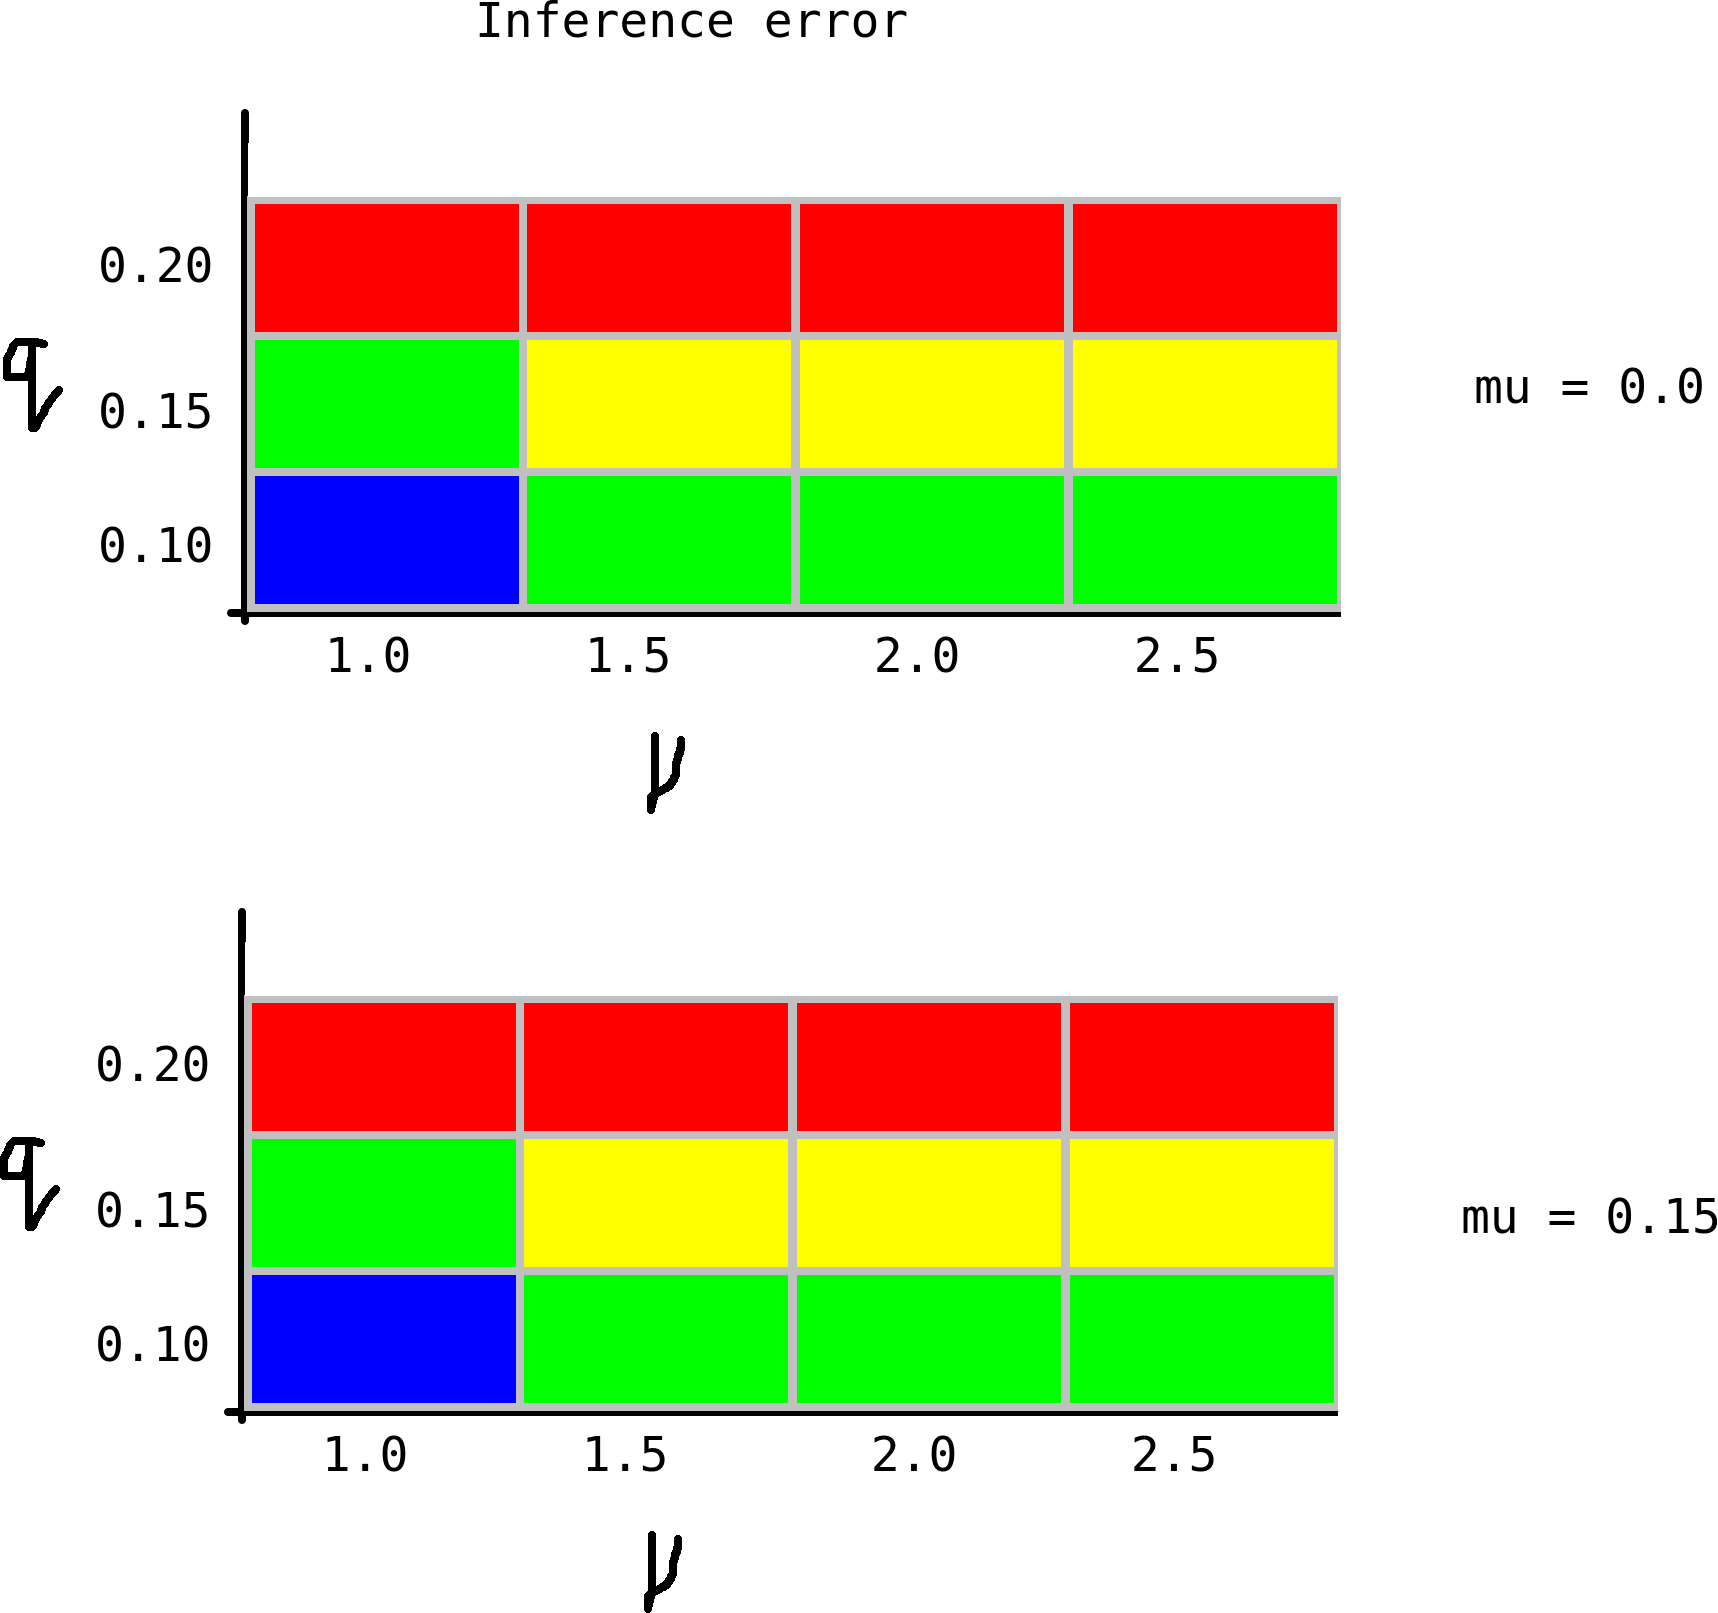
\includegraphics[width=\textwidth]{razzo-figures/fig_1.png}
  \caption{
    The inference error distribution (as indicated by the colors) 
    for the different biological
    parameter settings. In all cases, $\lambda = 0.2$ and 
    crown age equals 10. 
  }
  \label{fig:results}
\end{figure}

\bigskip\bigskip

\bibliographystyle{mee}
\bibliography{razzo-bibliography.bib}

\bigskip\bigskip

%%%%%%%%%%%%%%%%%%%%%%%%%%%%%%%%%%%%%%%%%%%%%%%%%%%%%%%%%%%%%%%%%%%%%%%%%%%%%%%%
\section{Supplementary materials}
%%%%%%%%%%%%%%%%%%%%%%%%%%%%%%%%%%%%%%%%%%%%%%%%%%%%%%%%%%%%%%%%%%%%%%%%%%%%%%%%

\begin{figure}[!htbp]
  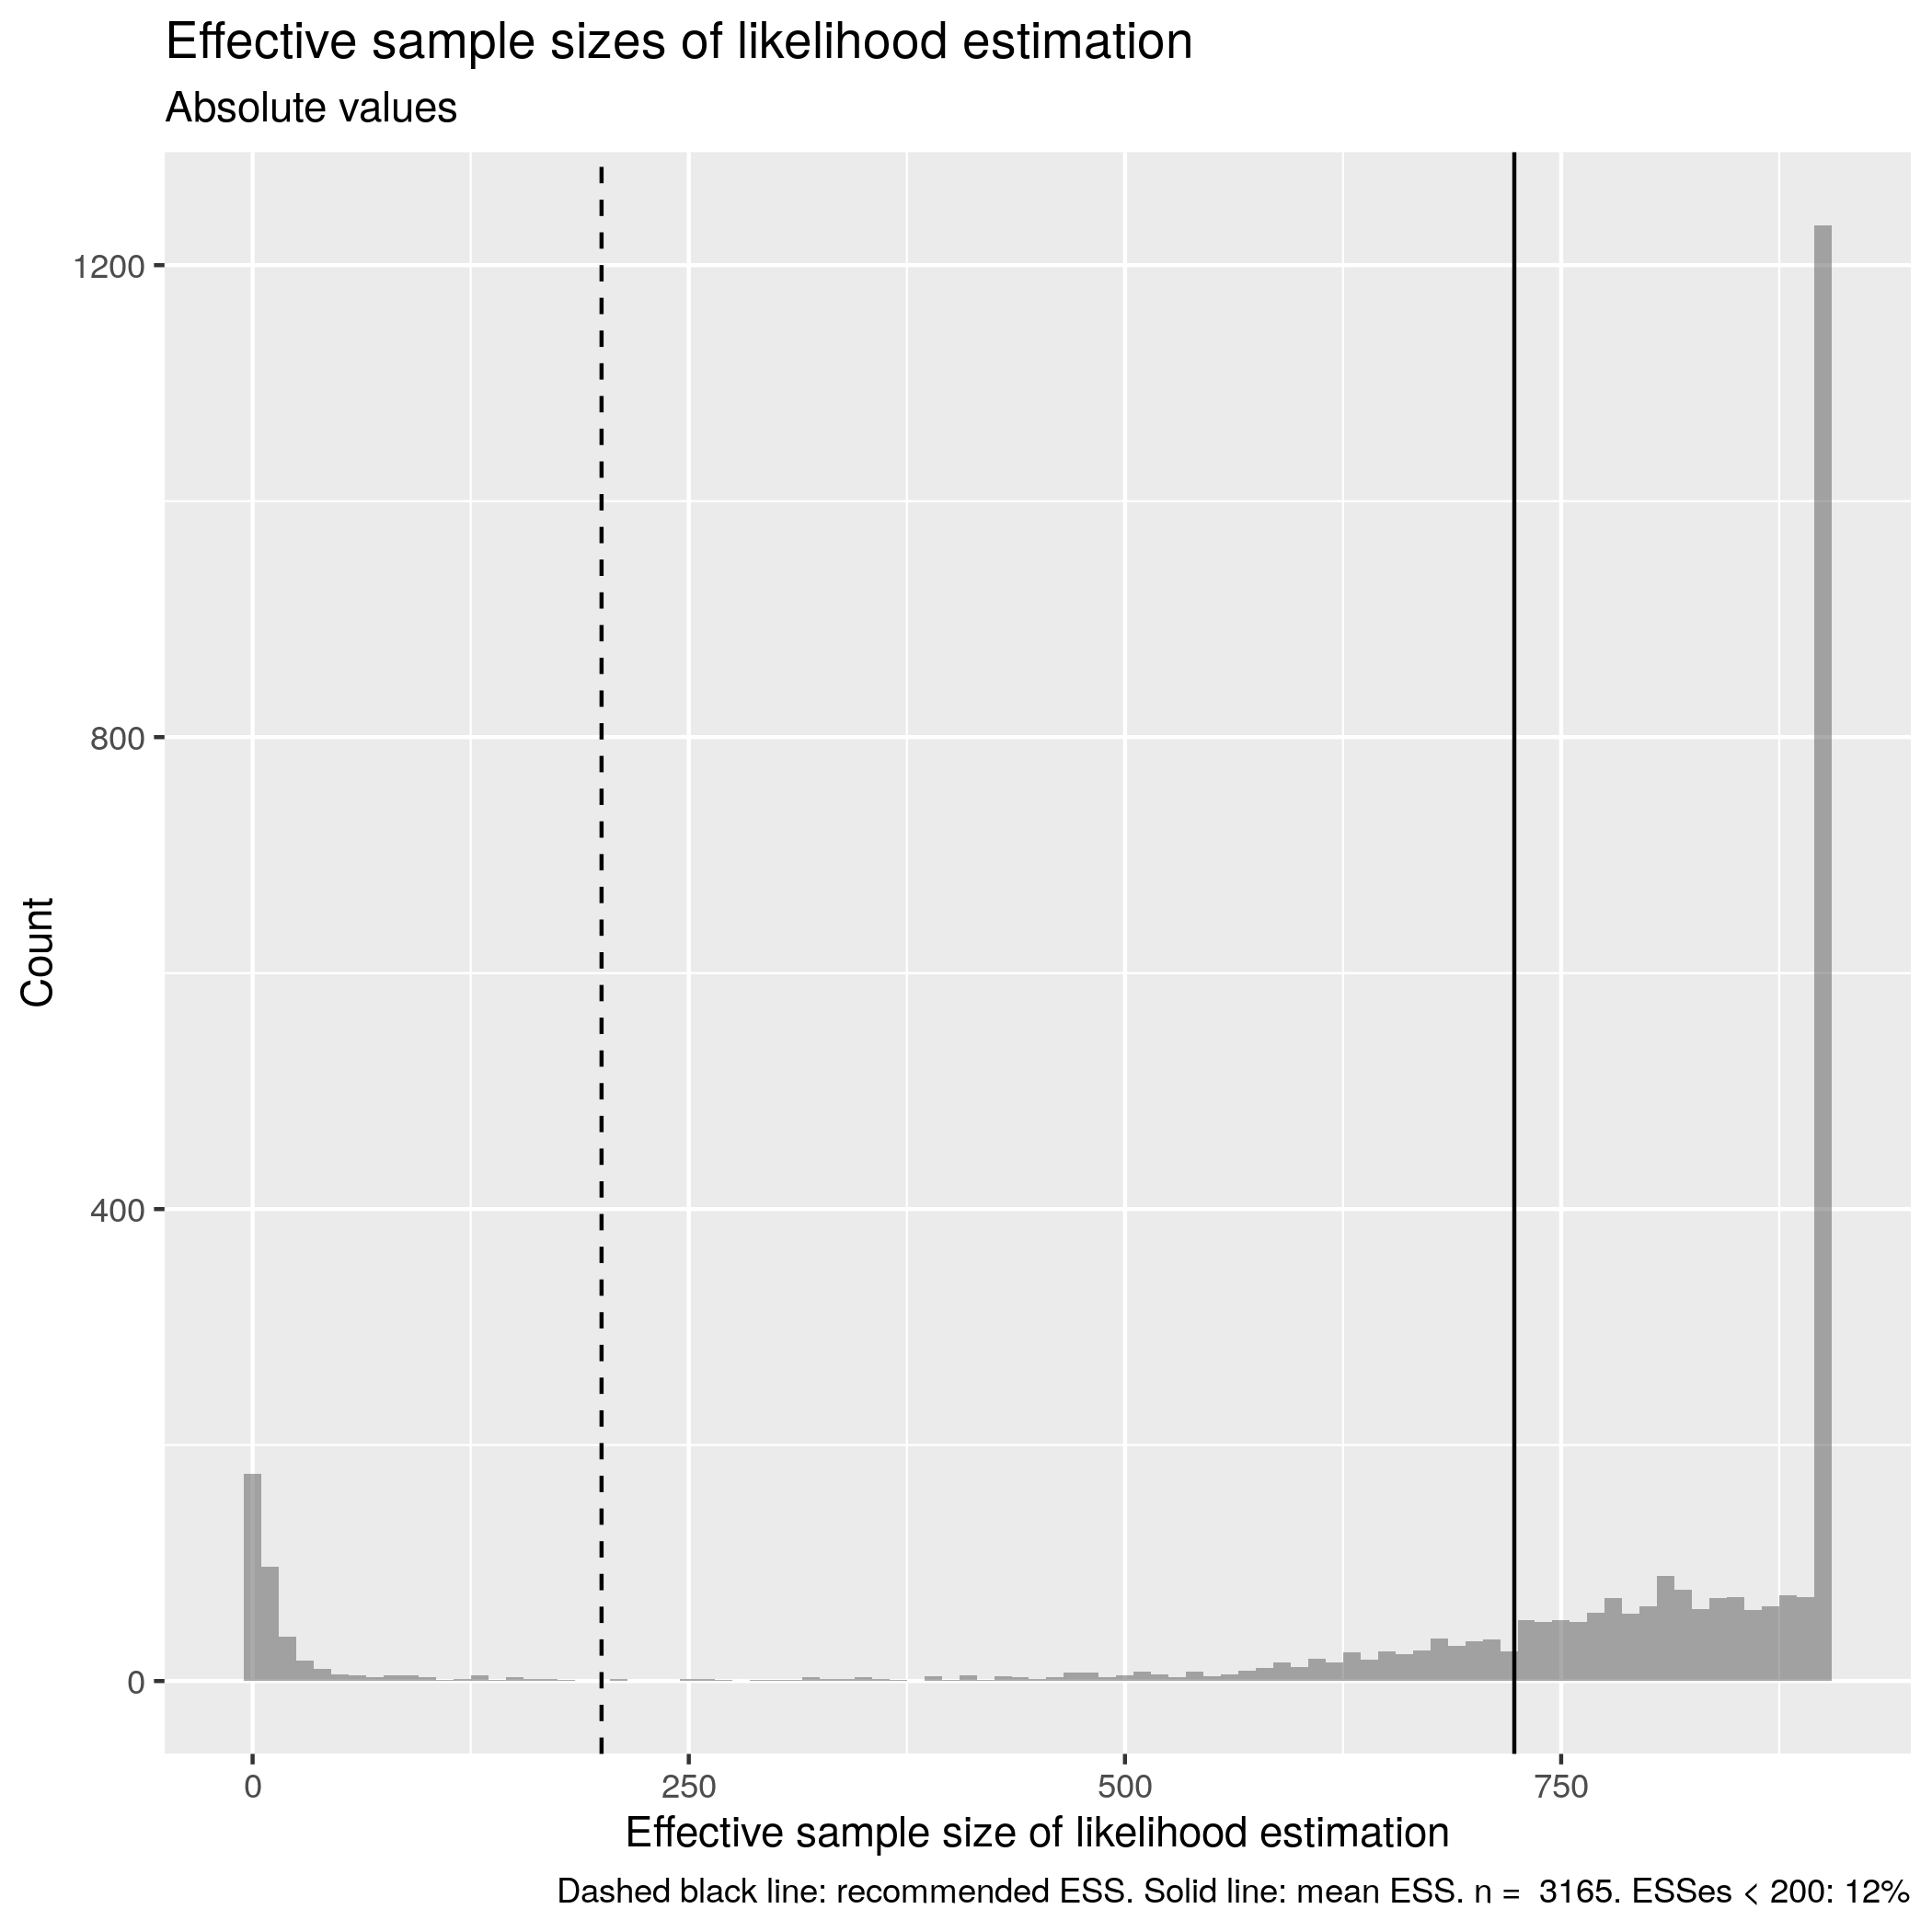
\includegraphics[width=\textwidth]{20200204_fig_esses.png}
  \caption{
    Effective sample sizes of the likelihood of all the experiments that
    finished within 10 days. 
    Each point is one parameter setting.
  }
  \label{fig:esses}
\end{figure}

\begin{figure}[!htbp]
  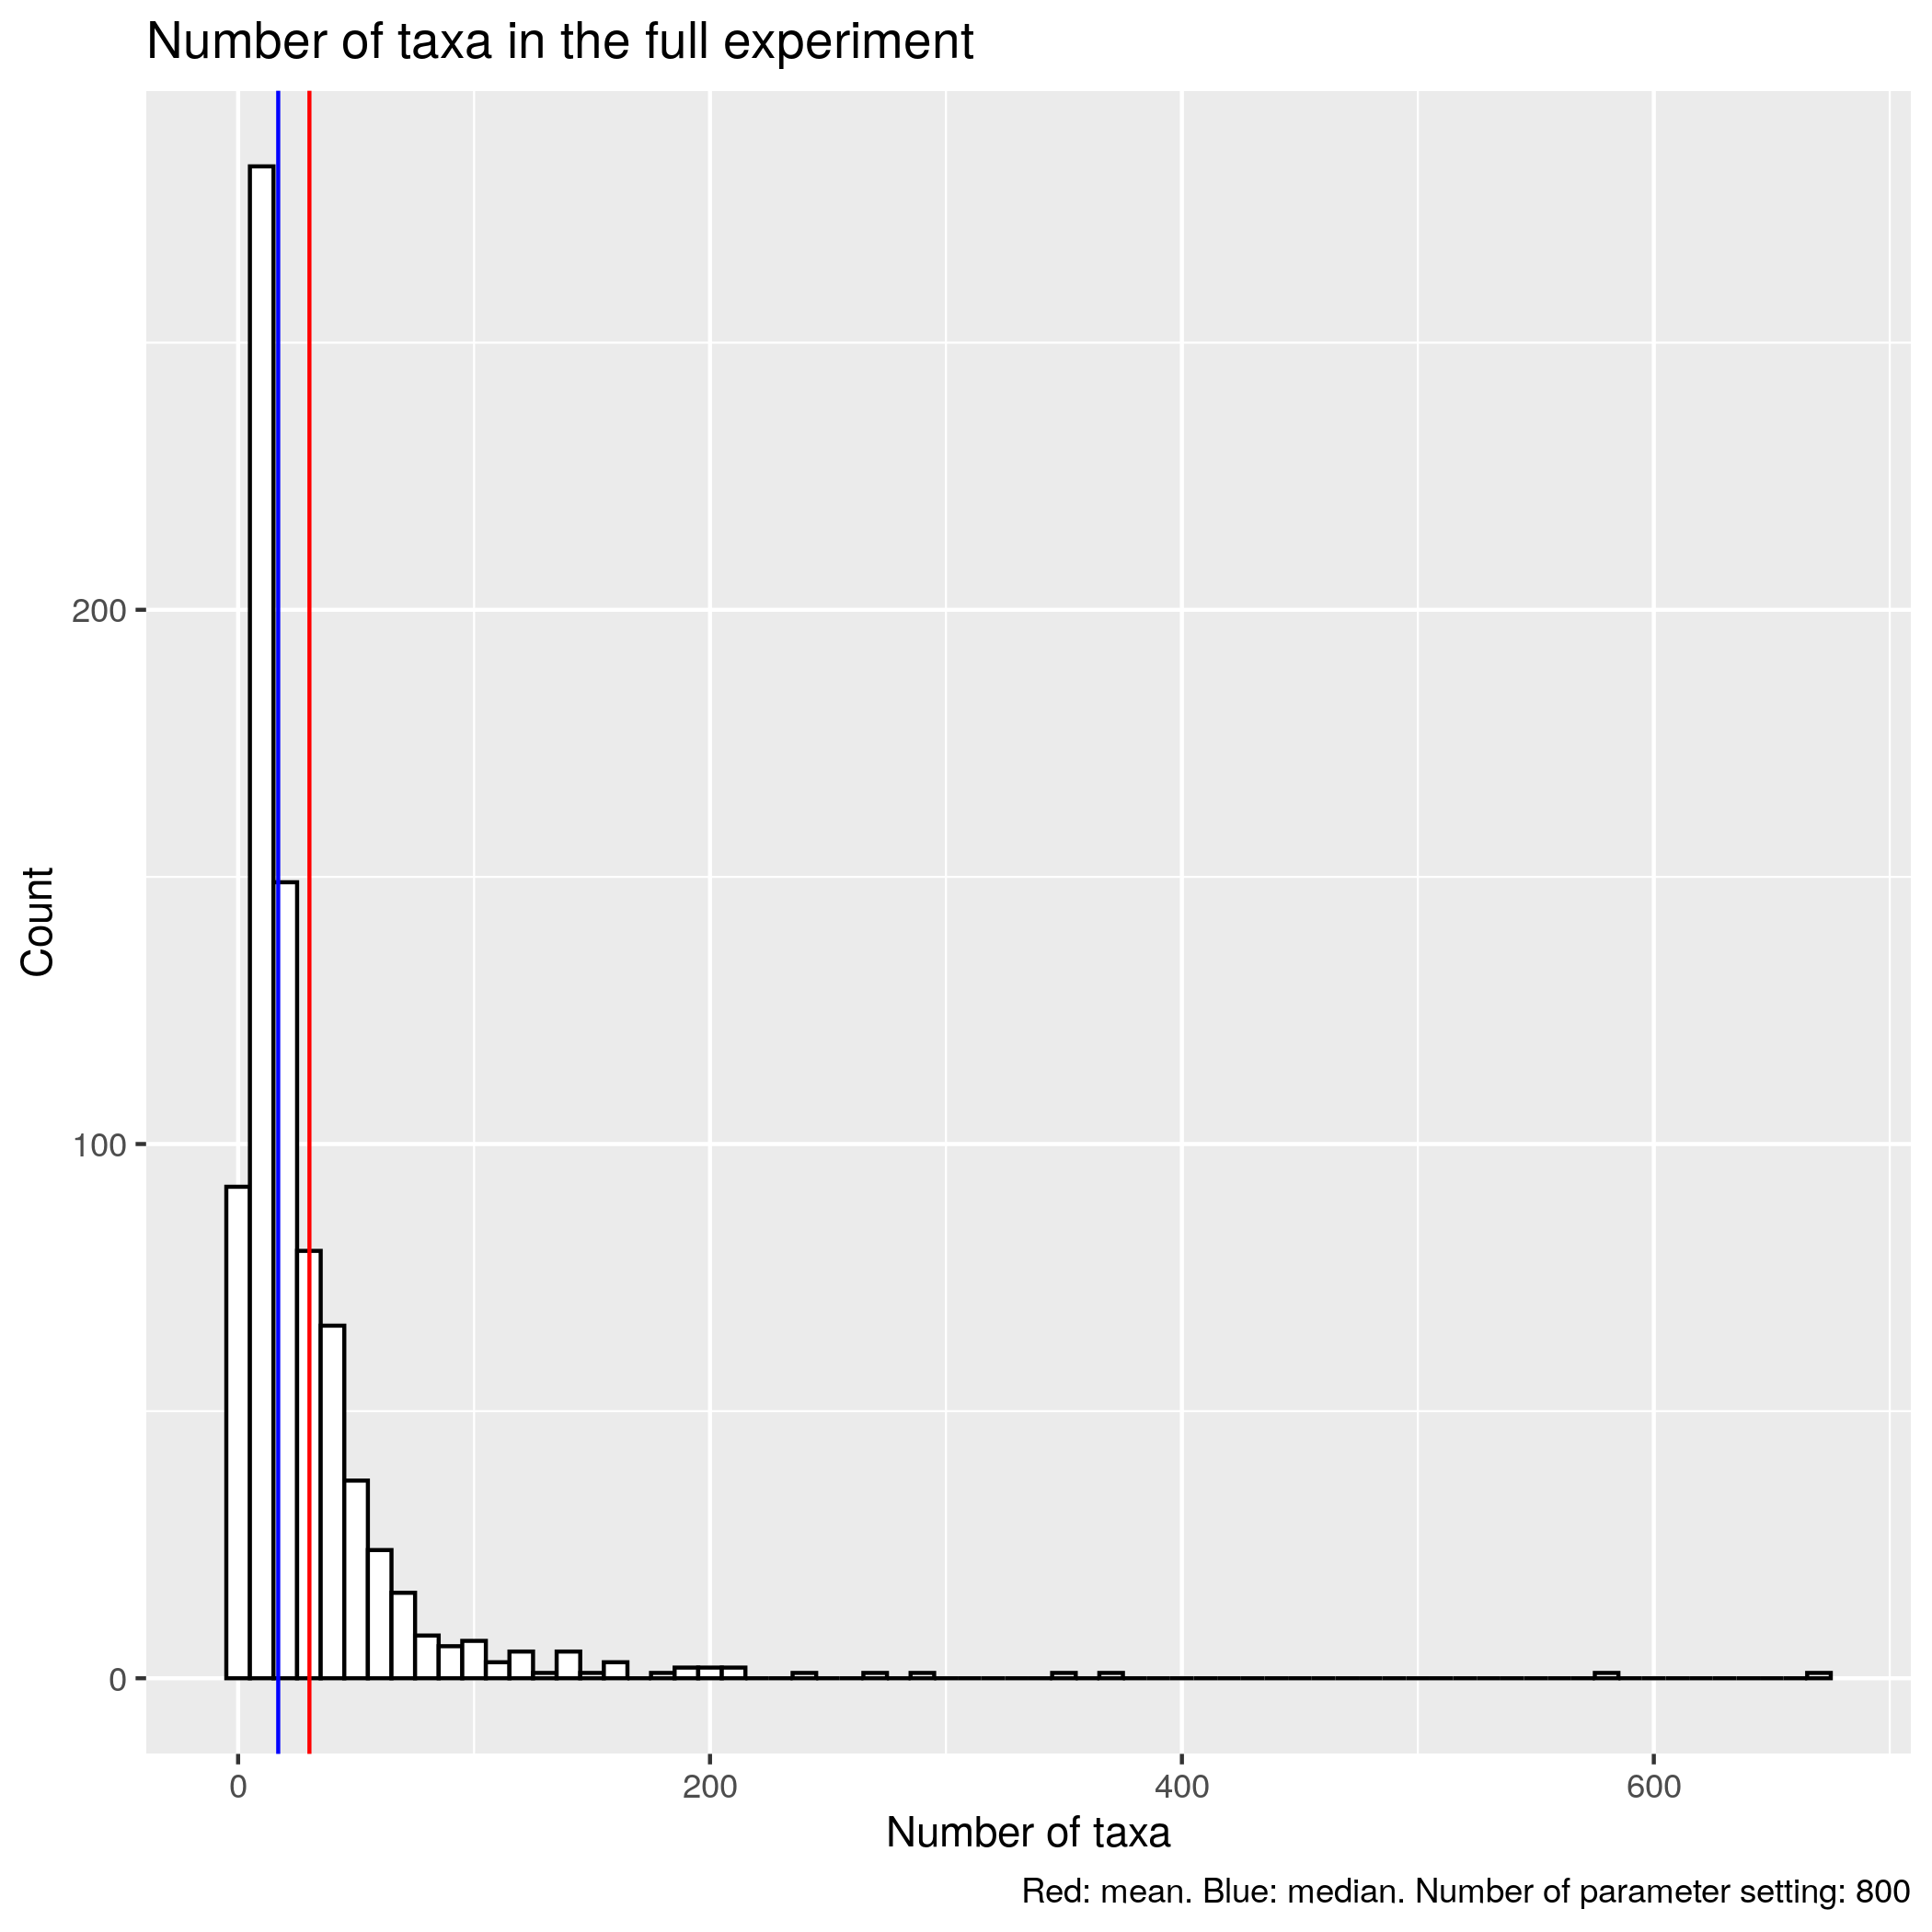
\includegraphics[width=\textwidth]{20200204_fig_n_taxa.png}
  \caption{
    Histogram of the number of taxa in the full experiment.
  }
  \label{fig:n_taxa}
\end{figure}

% 20200204_fig_marg_liks.png
% 20200204_fig_cumulative_esses.png
% 20200204_figure_1a.png
% 20200204_figure_1b.png
% 20200204_figure_1c.png
% 20200204_figure_1d.png



\end{document}
